\section{Теоретические сведения}
При нагреве частицы вещества начинают излучать электромагнитную энергию разных частот, совокупность которых называется \textit{спектром излучения} соответствующих частиц. Зависимость показателя поглощения вещества от длины волны проходящего через него излучения, соответственно, называется \textit{спектром поглощения} составляющих его частиц. В данной работе исследованы спектры некоторых атомов, а также двухатомных молекул йода.

\subsection{Излучение водородоподобных атомов}
Атом водорода является простейшей атомной системой, в связи с чем его спектральные свойства были тщательно изучены экспериментально и теоретически. Длины волн спектральных линий водородоподобного атома описываются формулой
\begin{equation}\label{hydrogen}
    \frac{1}{\lambda_{mn}} = RZ^2\left(\frac{1}{n^2} - \frac{1}{m^2}\right),
\end{equation}
где $n$~--- номер серии, $m$~--- целое число от $n+1$ до $+\infty$, а $R$~--- константа, называемая \textit{постоянной Ридберга}. Экспериментально установленное значение данной постоянной~--- $R = 109677,6$ см$^{-1}$.

\subsection{Спектр поглощения двухатомной молекулы йода}
Молекулы обладают более сложным спектром возбуждённых состояний, так как в них могут возбуждаться дополнительные степени свободны~--- вращательные, колебательные. При температуре, близкой к комнатной, спектр поглощения паров йода практически состоит из двух серий электронно-колебательного спектра~--- 0-й и 1-й \textit{серий Деландра}. Вид спектра и составлящих его серий изображён на рис.~\ref{fig:spectrum}.
\begin{figure}[h]
    \centering
    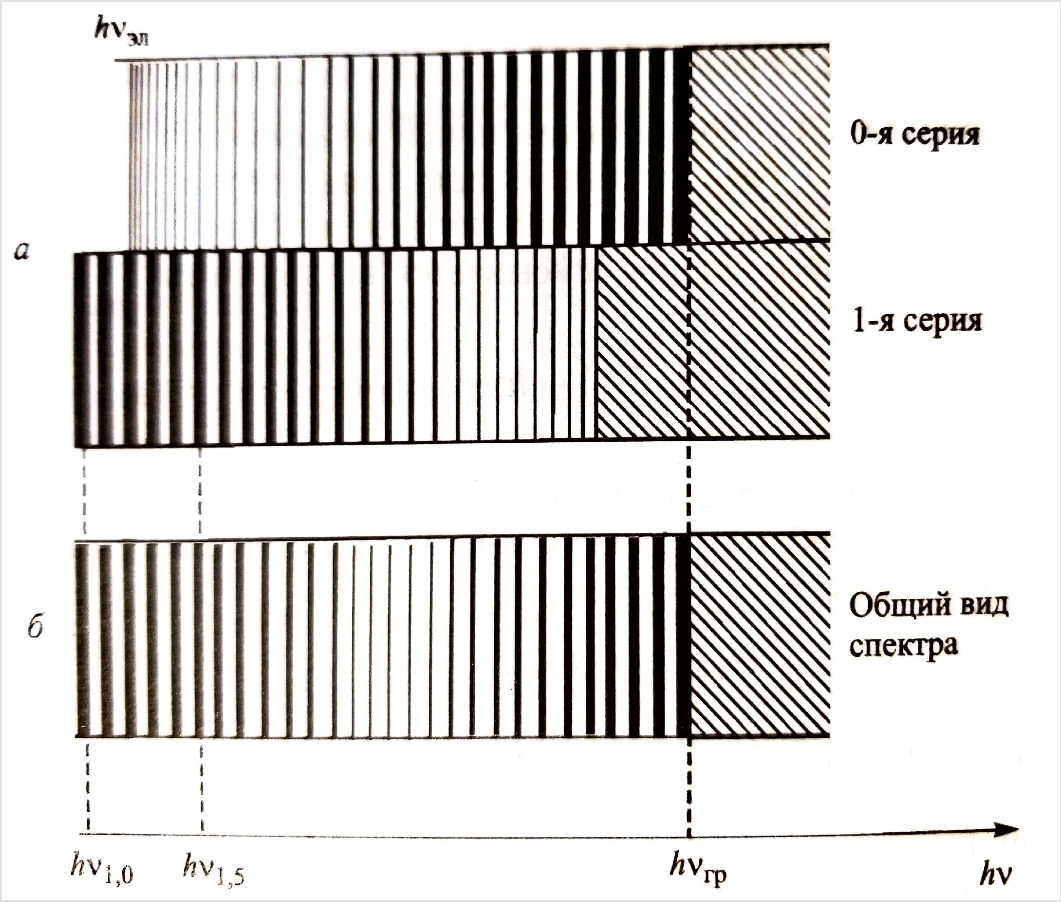
\includegraphics[width=0.45\textwidth]{img/spectrum.jpg}
    \caption{Спектр поглощения паров йода при $T\approx 300$ К}
    \label{fig:spectrum}
\end{figure}

Энергетическое положение начальных линий поглощения $n_1$-й серии определяется выражением
\begin{equation}\label{iodine1}
    h\nu_{n_1,\,n_2} = h\nu_\text{эл} + h\nu_2\left(n_2 + \frac{1}{2}\right) - \frac{1}{2}h\nu_1,
\end{equation}
где $n_2$~--- номер линии, $\nu_2$~--- соответствующая ей частота, $h\nu_1$~--- энергия колебательного кванта основного состояния, $h\nu_\text{эл}$~--- энергия электронного перехода. Расстояние между соседними линиями равно
\begin{equation}\label{iodine2}
    h\nu_{n_1,\,n_2} - h\nu_{n_1,\,(n_2 - 1)} \approx h\nu_2. 
\end{equation}
Здесь $n_2$~--- номер линии, $\nu_2$~--- соответствующая ей частота. Обозначим границу схождения спектра, то есть энергию возбуждения, при которой происходит переход молекулы в область непрерывного спектра, обозначим через $h\nu_\text{гр}$. Тогда энергии $D_1$ и $D_2$ диссоциации молекулы из состояний $n_1 = 0$ и $n_2 = 0$ соответственно выражаются как
\begin{equation}\label{iodine3}
    D_1 = h\nu_\text{гр} - E_a,\quad D_2 = h\nu_\text{гр} - h\nu_\text{эл},
\end{equation}
где $E_a$~--- энергия возбуждения атома.
